% Set the author and title of the compiled pdf
\hypersetup{
	pdftitle = {\Title},
	pdfauthor = {\Author}
}

\section{Introduction}
\subsection{A Computational Model}

The simplest, earliest, commonest, most important computational model is the
\textbf{Von-Neumann Imperative Procedural Computer Model}

According to this model, a computer can:
\begin{enumerate}
	\item Store information
	\item Manipulate the stored information
	\item Make decisions depending on the stored information
\end{enumerate}

\subsection{Simple View Of A Computer}
The simplest model of a computer can be represented as:

\[
	Memory \Leftrightarrow Bus \Leftrightarrow Processor
\]

\subsubsection{Memory}

Memory is a set of locations which can hold information, such as numbers,
programs or many other types of data. Each memory location has a unique
numerical address, and there are typically thousands of millions of different
locations. There are various ways of depicting memory; a common one is a 'hex
dump' that often looks something like this:

\begin{center}
	\begin{tabular}{l l l}
		{\bf Address}     &	{\bf Hex values}	&	{\bf ASCII}\\
		{\tt 00000000}	&	{\tt 48 65 6C 6C 6F 0A}		&	Hello.\\
	\end{tabular}
\end{center}

Each item that is in the memory has a unique address.

\marginpar{Run the command {\tt hexdump} to generate hexdumps.}

\subsubsection{Bus}

A bus is a bidirectional communication path. It is able to transmit addresses
and numbers between components inside the computer.

\subsubsection{Processor}

The processor obeys a sequence of instructions, commonly referred to as a
program. Historically the processor was often referred to as a CPU, however,
this is inappropriate nowadays since typical processors consist of several
processing cores.

\subsection{Three-address instructions}

Every kind of processor has a different set of instructions, real world examples
include: Pentium, ARM and others

Each three-address instruction:
\begin{enumerate}
	\item Copies the values from any two memory locations and sends them to the
	processor (source operands)
	\item Copies some operation e.g. adds the copied numbers together
	\item Copies the result back from the processor into a third memory location
	(destination operand)
\end{enumerate}

For example, if we wanted to convert the Java code {\tt sum = a + b;} into a
three-address instruction we would:

\begin{enumerate}
	\item Identify the two {\it source operands}: $a$ holds 2, $b$ holds 3
	\item Perform the {\it operation}: 2 + 3 = 5
	\item Let the variable $sum$ equal the answer 5. This is the {\it 
	destination operand}
\end{enumerate}

\subsubsection{Three address example}

{\bf Question:} Convert the Java code {\it product = c * d;} into the three-
address style and draw a two box view of it.

First we need to re-write the Java code in the three-address style:
\[
	product \leftarrow c * d
\]
Now we can draw the box view of it (figure~\ref{figure:two_box_model}).

\begin{figure}[ht!]
	\centering
	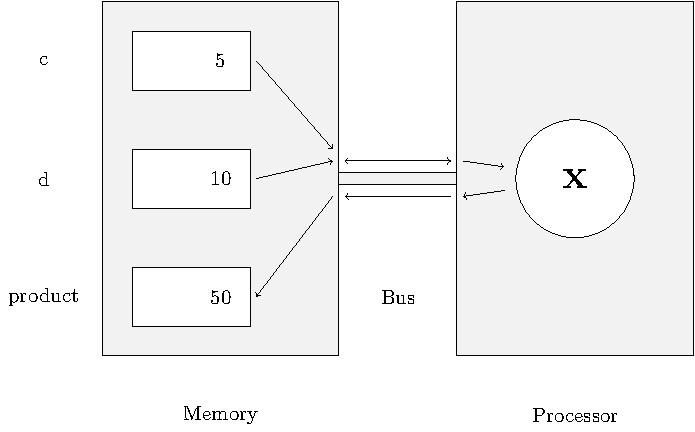
\includegraphics[width=\textwidth]{two_box_model_diagram.pdf}
	\caption{An example of the two box model}
	\label{figure:two_box_model}
\end{figure}

\subsubsection{Memory bottleneck}

Most processors can process instructions faster than they can be fed by memory.
Each instruction in the three-address cycle requires four memory cycles:

\begin{enumerate}
    \item Fetch the instruction
    \item Read the first operand
    \item Read the second operand
    \item Write the result to memory
\end{enumerate}

Each of these memory cycles could take hundreds of processor clock cycles to
complete, and so in this time the processor would be doing nothing. However,
most modern processors employ a {\it cache} to temporarily store commonly
accessed memory locations, and so avoid some of the memory cycles.

\subsection{Registers}

Registers are very small amounts of storage build into a processor. Since they
are inside the processor data doesn't need to be transferred over the bus, and
so they are very fast. Registers are used instead of the main memory which
speeds up program execution.

Each register can only hold one value and each processor will only generally
have a few dozen registers (e.g. ARM has sixteen).

\subsection{Instruction Styles}

\subsubsection{One address}

The one address style can only use up to one memory location in each
instruction, all other operands must be registers. An example may be:

\[
    R1 \leftarrow R0 + \textrm{\it memory location}
\]

\subsubsection{Load-store}

The load-store style cannot perform operations on memory locations at all.
Instead, values from memory must be loaded into a registers before the operation
takes place and then the operation can be performed on the registers. Following
the operation, the result must be stored back into memory again.

\[
	\begin{split}
	    R1 &\leftarrow \textrm{\it memory location}\\
		R1 &\leftarrow R0 + R1\\
	    \textrm{\it memory location} &\leftarrow R1
    \end{split}
\]

This means that we need extra instructions to do stuff with memory locations:
\begin{enumerate}
	\item \textbf{Load} the value from memory into a register before the 
	operation.
	\item \textbf{Store} the value in the register back to memory after the 
	operation.
\end{enumerate}

For example, the Java code {\it Sum = a + b + c;} would be run as:

\begin{center}
    \begin{tabular}{l l l r}
        R1 & $\leftarrow$ & a & (i.e. load from a)\\
        R2 & $\leftarrow$ & b & (i.e. load from b)\\
        R3 & $\leftarrow$ & R1 + R2 & (i.e. a+b)\\
        R4 & $\leftarrow$ & c & (i.e. load from c)\\
        R5 & $\leftarrow$ & R3 + R4  & (i.e. (a+b)+c)\\
        Sum & $\leftarrow$ & R5 & (i.e. store to sum)\\
    \end{tabular}
\end{center}

You can see that the load-store style favours lots of very simple, very fast
instructions.

% This subsection was lifted straight from the COMP111 notes
% TODO: Figure out a way to make this subsection *cleanly* use the same source
%       file as the subsection in COMP111?
\subsection{An introduction to bases}

Conventionally, we count using base 10. Base 10 includes, you guessed it, ten
different symbols from 0 through to 9.

Sometimes however, it is convenient to count using different bases. Popular
bases include:

\begin{center}
	\begin{tabular}{l l l}
		{\bf Base $n$} & {\bf Member symbols} & {\bf Name}\\
		$n = 2$ & $\mathbb{Z}_2 = \{0, 1\}$ & Binary\\
		$n = 8$ & $\mathbb{Z}_8 = \{0, 1, 2, 3, 4, 5, 6, 7\}$ & Octal\\
		$n = 10$ & $\mathbb{Z}_{10} = \{0, 1, \ldots, 7\}$ & Decimal\\
		$n = 16$ & $\mathbb{Z}_{16} = \{0-9, A-F\}$ & Hexadecimal\\
	\end{tabular}
\end{center}

\subsubsection{How to read numbers in any given base}

The formula for reading a number in a given base is as follows:

\begin{dmath*}
	\sum_{i=0}^{k}a_{i}b^{i}
\end{dmath*}

Where the number you're trying to read takes the form $a_k, a_{k-1}, \ldots,
a_2, a_1, a_0$, $b$ is the base you're using and $i$ is the count from right
to left of the digits in the number.

\paragraph{Example 1}

Lets apply the formula to the base 10 number {\tt 27385}:

\begin{dmath*}
		27385 = (5 \times 10^0) + (8 \times 10^1) + (3 \times 10^2) +
				(7 \times 10^3) + (2 \times 10^4)
		      = (5 \times 1) + (8 \times 10) + (3 \times 100) + 
		      	(7 \times 1000) + (2 \times 10000)
		      = 5 + 80 + 300 + 7000 + 20000
		      = 27385
\end{dmath*}

\paragraph{Example 2}

Lets apply the formula to the base 16 number {\tt F00BA4}:


\begin{dmath*}
	F00BA4 = (4 \times 16^0) + (A \times 16^1) + (B \times 16^2) +
			 (0 \times 16^3) + (0 \times 16^4) + (F \times 16^5)
	       = (4 \times 16^0) + (10 \times 16) + (11 \times 256) +
	       	 (0 \times 4096) + (0 \times 65536) + (15 \times 1048576)
	       = 4 + 160 + 2816 + 0 + 0 + 15728640
	       = 15731620
\end{dmath*}

\subsubsection{Changing from base 10 to base $n$}

In order to change into base $n$ from base 10, we just repeatedly divide by $n$
and use the remainder as the value for base $n$. Here are a few examples:

\paragraph{Example 1}
Convert 893 into base 2.

\begin{center}
	\begin{tabular} {r l l l }
		$893 \div 2$ & = & 446 & r1\\
		$446 \div 2$ & = & 223 & r0\\
		$223 \div 2$ & = & 111 & r1\\
		$111 \div 2$ & = & 55 & r1\\
		$55 \div 2$ & = & 27 & r1\\
		$27 \div 2$ & = & 13 & r1\\
		$13 \div 2$ & = & 6 & r1\\
		$6 \div 2$ & = & 3 & r0\\
		$3 \div 2$ & = & 1 & r1\\
		$1 \div 2$ & = & 0 & r1\\
	\end{tabular}
\end{center}

Reading up from the bottom, we can see that the binary (base 2) representation
is $1101111101$.

\paragraph{Example 2}
Convert 893 into base 9.

\begin{center}
	\begin{tabular} {r l l l }
		$893 \div 9$ & = & 99 & r2\\
		$99 \div 9$ & = & 11 & r0\\
		$11 \div 9$ & = & 1 & r2\\
		$1 \div 9$ & = & 0 & r1\\
	\end{tabular}
\end{center}

Reading up from the bottom, we can see that the nonal (base 9) representation is
$1202$.

\paragraph{Example 2}
Convert 893 into base 16.

\begin{center}
	\begin{tabular} {r l l l }
		$893 \div 16$ & = & 55 & r13\\
		$55 \div 16$ & = & 3 & r7\\
		$3 \div 16$ & = & 0 & r3\\
	\end{tabular}
\end{center}

Reading up from the bottom, we can see that the hexadecimal (base 16)
representation is $3,7,13$ or $37D$.


\section{ARM}

Computers obey programs which are sequences of instructions. Instructions are
coded as values in memory. The sequences are held in memory adjacent memory
locations. Values in memory can be interpreted as you please, from numbers to
text, images or anything really!

Any given set of binary digits can be read as a decimal number, but not always
as text, so values in memory are often represented as numbers for convenience.

\subsection{Assembly Language}

Assembly language is a means of representing machine instructions in a human
readable form.

Each type of processor has its own assembly language (since each language is
specific to a particular architecture) but each instruction typically has a lot
in common:

\begin{itemize}
	\item A mnemonic, that specifies the type of operation
	\item A destination, such as a register or memory location
	\item And one or more sources that may be registers or memory locations.
	\item Possibly with a comment too which will help programmers understand 
	what's happening and aren't interpreted by the assembler.
\end{itemize}

When a program has been written in assembler, it must be {\it assembled} by an
{\it assembler} to run it.

\subsection{ARM instructions}

ARM has many instructions but we only need three categories:

\begin{itemize}
	\item Memory operations that move data between the memory and the registers.
	\item Processing operations that perform calculations using value already in
	registers.
	\item Control flow instructions are used to make decisions, repeat 
	operations etc.
\end{itemize}

\subsection{Transferring data between registers and memory}

Memory operations load a value into a register from an address in memory or
store the value of a register to a memory address.

For example, $a$ into register 1 ($R1 \leftarrow a$) we would write:
{\tt LDR R1, a}

Or to store the value in register 5 into $sum$ ($sum \leftarrow R5$):
{\tt STR R5, sum}

In these examples, $a$ and $sum$ are aliases for the addresses of memory
locations.

\subsection{ARM processing instructions}

ARM has many different instructions to perform operations such as addition,
subtraction and multiplication.

The syntax for such operations is usually:

\begin{verbatim}
	[operand]	[destination register]	[register 1]	[register 2]
\end{verbatim}

For example, to add two numbers together, we might write:

\begin{verbatim}
	ADD	R2, R0, R1
\end{verbatim}

This will add the value of R0 to the value of R1 and store it in R2.

\subsection{ARM control instructions}

The most common control instruction is the branch. Similar to \texttt{GOTO} in
other languages, a branch will change the PC register (see
section~\ref{subsec:pc}) to another value so the order of execution of the
program is changed.

Branches can be made to be conditional by appending a conditional operator on to
the command.

The syntax is something like:

\begin{verbatim}
	B[conditional operator]	[branch name]
\end{verbatim}

Some examples of different conditional operators are:

\begin{tabularx}{\textwidth}{l X}
	{\bf Command} & {\bf Function}\\
	\texttt{B} & Branches to a different location in the code.\\
	\texttt{BNE} & Branches, but only if the previous condition was false.\\
	\texttt{BEQ} & Branches, but only if the previous condition was true.\\
\end{tabularx}

\subsection{Stored programs and the Program Counter}
\label{subsec:pc}

A computer can make decisions, and choose which instructions to obey next
depending upon the results of those decisions. A {\bf Program Counter} (PC)
register is used to hold the memory address of the next instruction to be
executed. ARM uses register 15 as its PC.

\subsection{Fetch-Execute Cycle}

The processor must first fetch instructions from memory before it can execute
them. This is called the fetch-execute cycle, and it involves:

\begin{enumerate}     \item \textbf{Fetch}: copy the instruction, pointed to by
the PC, from memory and set PC to point to the next instruction     \item
\textbf{Execute}:  obey the instruction (exactly as before)     \item Repeat.
\end{enumerate}

In ARM, the PC starts with a values of \texttt{0x00000000} when the program is
initially run. On each cycle of the Fetch-Execute cycle, the PC is incremented
by 4, since instructions each occupy 4 memory locations.

\subsection{Decision Making}

In order to make decisions, the computer mustn't just execute instructions one
after the other in a linear manner. Instead, branches must be used to change the
sequence of instructions to be executed.

In order to perform a conditional branch, we must first perform a compare
command to perform the comparison before we do the branch.

\subsubsection{An example}

If we wanted to do a $£1$ discount on a shopping list if the price was over
$£20$, we would do the following:

\begin{listing}{1}
		LDR	R0, total	; Load the total price
						; into R0
	
		CMP	R0, #20		; Compare R0 and 20
						; (the literal)
		BLT	nodiscount	; If the price is too low,
						; then don't discount
		SUB	R0, #1		; Deduct £1
		STR	R0, total	; Store the result back 
						; into memory

nodiscount	SVC	2		; Finish

total 		DEFW	25		; Lets say the total is \$25
\end{listing}

\subsection{Allocating memory}

The \texttt{DEFW} (define word) operation puts a value in memory before the
program is run. Any define operation is executed before the program is run.

The actual memory location that is used to store the value isn't known to the
running program, however, an {\it alias} is attached to the memory location by
the programmer and the memory location can be referenced through that.

The syntax for the \texttt{DEFW} command is as follows:

\begin{verbatim}
myage	DEFW	18
\end{verbatim}

Where {\tt myage} is the alias and {\tt 18} is the value.

{\tt DEFW} can also be used to define a number of words:

\begin{verbatim}
squares	DEFW	0, 1, 4, 9, 16, 25
\end{verbatim}

\marginpar{The label ({\tt squares}) is associated with the lowest address (i.e.
0)}

{\tt DEFB} stores a single byte in memory. It is useful for strings such as
"hello":

\begin{verbatim}
hi	DEFB	"hello"
\end{verbatim}

{\tt DEFS} sets a block of bytes to a set value:

\begin{verbatim}
reserved_space	DEFS	10, 5
\end{verbatim}

The above will set 10 bytes to the value '5'.

\section{Storing values}

% TODO: Expand on this section

There are many ways to store data. For example, we could store what lights are
one in a traffic light in many different ways. First, we must decide how many
different states the traffic light can be in:

\begin{verbatim}
	Red, Red Amber, Green, Amber
\end{verbatim}

You can see that we have four states. This could be represented in binary as two
bits:

\begin{center}
	\begin{tabular}{|c|c|}
		\hline
		{\tt 00} & Red\\ \hline
		{\tt 01} & Red Amber\\ \hline
		{\tt 10} & Green\\ \hline
		{\tt 11} & Amber\\ \hline
	\end{tabular}
\end{center}

We could also store the states as their binary representations of their names:

\begin{center}
	\begin{tabular}{|c|c|}
		\hline
		R & {\tt 01010010}\\ \hline
		RA & {\tt 0101001001000001}\\ \hline
		G & {\tt 01000111}\\ \hline
		A & {\tt 01000001}\\ \hline
	\end{tabular}
\end{center}

You can see though, that this isn't as efficient as storing just two binary
digits.

\section{ARM assembly programming}

\subsection{Different types of values}

ARM has the capacity to work with many different types and sizes of values. Each
type has a different use case. The main ones are described below:

\begin{tabularx}{\textwidth}{l l X}
	{\bf Name} & {\bf length} & {\bf Use}\\
	Byte & 8 bits & Used for characters\\
	Word & 32 bits & Used for integers, addresses and instructions\\
\end{tabularx}

There are other types too (such as the halfword and doubleword) but they aren't
needed for this module.

ARM processors require that memory locations are aligned. This means that values
stored in memory start at specific places. For example, a word address must be a
multiple of four.
e
This means that after a {\tt DEFW} statement, the {\tt ALIGN} command must be
called (See ~\ref{subsubsec:align} for more on the {\tt ALIGN} command.).

\subsection{Loading and storing values in memory}

The commands {\tt LDR} and {\tt STR} are used to move values between memory and
registers. The commands are detailed in full below:

\begin{tabularx}{\textwidth}{l X}
	{\bf Command} & {\bf Function}\\
	{\tt STR} & Copies the whole (32 bit) register into memory.\\
	{\tt LDR} & Loads a 32 bit word from memory into a register.\\
	{\tt STRB} & Stores a single 8 bit byte into memory from a register.\\
	{\tt LDRB} & Loads a byte from memory into a register. The upper 24 bits of
	the register are zeroed.\\
\end{tabularx}

\subsection{Endianness}

Endianness is a property of a memory location that defines the order of the
bits. There are two types of endianness, {\bf little endian} and {\bf big
endian}.

In the word {\tt 0x12345678} there are four bytes:
\begin{itemize}
	\item {\tt 0x12}
	\item {\tt 0x34}
	\item {\tt 0x56}
	\item {\tt 0x78}
\end{itemize}

In little endian, the first byte would be {\tt 0x12} since bits are read from
right to left in little endian.

In big endian, the first byte would be {\tt 0x78} since bits are read from left
to right in big endian.

This is important when we deciding what the most and least significant bits in a
word are. For example, in this instance the {\it lsb} is {\tt 0x12} in little
endian, but {\tt 0x78} in big endian.

In this course, little endian is used, though ARM can use either.

\marginpar{N.b. The least significant bit is the smallest address. It is the one
that has a value of {\tt 1} and thus determines if the number is odd or even.}

\subsection{Addressing memory}

ARM uses 32 bit addresses, so there are $2^{32}$ different bytes that can be
addressed in memory (or $\frac{2^{32}}{4}$ different words). However, there is
no guarantee that the system on which the program is running will have that much
memory available.

\subsection{Instruction encoding}

Each ARM instruction is encoded into a four byte word. The exact meaning of each
of the bits varies per instruction.

For example, in the branch instruction, the first four bits specify the
condition, the second four bits represent the actual operation to perform (i.e.
branch) and the remaining twenty four bits define the memory location of the
next instruction to branch to.

However, this presents a problem. We only have twenty four bits with which to
define the next location to branch to, which allows us to define $2^{24}$
different locations. However, there are $2^{32}$ possible addresses that we
could use!

This problem is overcome by treating the 24 bits as an offset to the address of
the current instruction. This works since most of the time, the address that is
being branched to is fairly close to the current instruction.

In order to be able to branch to addresses before and after the current
instruction, we must use two's complement to allow signed integers to be used to
specify the offset. This means we can branch to any instruction at an address
$\pm 2^{23}$ from the current instruction.

\subsection{Literals}

ARM is able to encode literal values into instructions. This saves time having
to access registers or memory in order to perform operations such as arithmetic.

An example is to increment a register:

\begin{verbatim}
	ADD	R1, R1, #1
\end{verbatim}

However, ARM only assigns up to 12 bits for a literal value, so we can only have
$2^{12}$ values. However, ARM employs a strange method of encoding these values
so that more useful values are available (for example, \#512 is allowed, but
\#257 isn't).

\subsubsection{Negative literals}

Technically, ARM doesn't support negative literals, however, the assembler will
usually be able to find a way to implement them. Some examples are given below:

\begin{center}
    \begin{tabular}{l l l r}
        {\tt ADD R1, \#-1} & $\rightarrow$ & {\tt SUB R1, \#1}\\
        {\tt CMP R2, \#-2} & $\rightarrow$ & {\tt CMN R2, \#2}\\
        {\tt MOV R3, \#-3} & $\rightarrow$ & {\tt MVN R3, \#3}\\
    \end{tabular}
\end{center}

\marginpar{{\tt CMN} is compare negative.\\{\tt MVN} is move not.}

\subsection{Supervisor calls}

Supervisor calls are functions implemented by the operating system, not ARM
itself. The parameter of an {\tt SVC} call defines it's exact
operation.

\marginpar{{\tt SWI} is the old (yet still occasionally used) command for
{\tt SVC} - they do the same thing. {\tt SWI} stands for 
{\it SoftWare Interrupt}, and {\tt SVC} stands for {\it SuperVisor Call}}

In this module, the SVC call does the following for each parameter:

\begin{tabularx}{\textwidth}{l X}
	{\tt SVC 0 } & Output a character \\
	{\tt SVC 1 } & Input a character \\
	{\tt SVC 2 } & Stop execution \\
	{\tt SVC 3 } & Output a string \\
	{\tt SVC 4 } & Output an integer \\
\end{tabularx}

\subsection{Pseudo instructions}

The ARM assembler provides some instructions that are translated into sequences
of more complicated instructions at the time of assembly for our convenience.

One such instruction is loading a literal into a register. This is done using
the {\tt LDR} command as usual, however a literal is used with the '$=$'
character instead of a '$\#$'. E.g. to load the value $100$ into register one,
we do:

\begin{verbatim}
	LDR	R1,	=100
\end{verbatim}

However, this is a pseudo instruction and will be converted by the assembler to:

\begin{verbatim}
	MOV	R1,	#100
\end{verbatim}

However, if the number is very large, it becomes:

\begin{verbatim}
constant	DEFB	100
		LDR	R1, constant
\end{verbatim}

\subsection{Loading an address into a register}

The {\tt ADR} command loads an address into a register, for example:

\begin{listing}{1}
constant	DEFB	100
		ADR	R1, constant
\end{listing}

It will load the memory address of {\tt constant} relative to the {\tt PC} into
{\tt R1}. When the code is assembled, it is turned into two instructions (so
{\tt ADR} is a pseudo instruction). They are:

\begin{listing}{1}
	ADD R1, R1, PC
	LDR PC, R1
\end{listing}

\subsection{Directives}
Directives are evaluated at the time of assembly.

\subsubsection{DEF commands}

The {\tt DEF\{W,B,S\}} command reserves an amount of memory dependent on the
operation used (see the table) and puts an initial value in it.

\begin{tabularx}{\textwidth}{l|X}
	{\bf Command} & {\bf Function}\\ \hline

	{\tt DEFW num} & Reserves a {\it word} of memory and puts the initial
	value {\tt num} in it.\\ \hline

	{\tt DEFB value} & Reserves {\it byte}(s) of memory and puts the initial
	value {\tt value} in it. Note that the value can be a string literal, in
	which case the number of bytes reserved will be equal to the length of the
	string.\\ \hline

	{\tt DEFS size, fill} & Reserves a {\it block} of memory of {\tt size}
	bytes and initialises them with the value {\tt fill}. \\ \hline	
\end{tabularx}

\subsubsection{Align}
\label{subsubsec:align}

The align command leaves as many blank bytes as needed so that the next item in
memory will start at a word boundary (a multiple of 4).

\subsubsection{Entry}

Sets the PC at the start of the program (i.e. where the program should start
from)

\subsubsection{EQU}

Allows you to name a literal, which can go a long way to making the code more
maintainable. We could define the literal $18$ as $drinking\_age$:

\begin{listing}{1}
drinking_age	EQU 	#18
		; Check the person is over 18
		CMP 	R1, #drinking_age
		BLT	too_young
\end{listing}

\section{Arithmetic}

\subsection{Making good use of registers}

Registers are a precious resource when programming on ARM. When writing software
to evaluate expressions, it's often tempting to load all the variables into
registers first, and then perform the arithmetic in separate registers like so:

\begin{listing}{1}
	; a = b + c + d
	LDR 	R1, b
	LDR 	R2, c
	LDR 	R3, d
	ADD 	R4, R1, R2
	ADD 	R5, R4, R3
	STR 	R5, a
\end{listing}

However, this is pointless - the values in the registers {\tt R4} and {\tt R5}
aren't going to be needed again, so we may as well do:

\begin{listing}{1}
; a = b + c + d
LDR 	R1, b
LDR 	R2, c
LDR 	R3, d
ADD 	R1, R1, R2
ADD 	R1, R1, R3
STR 	R1, a
\end{listing}

But, we can optimise even further here. Instead of loading all the variables
into registers before we do arithmetic, we can save a register and load only the
ones we need before each {\tt ADD} instruction:

\begin{listing}{1}
; a = b + c + d
LDR 	R1, b
LDR 	R2, c
ADD 	R1, R1, R2
LDR 	R2, d
ADD 	R1, R1, R2
STR 	R1, a
\end{listing}

Sometimes, it's useful to re-order an arithmetic expression so it can be
implemented using less registers. This can often be achieved by increasing the
nesting of brackets in an expression such as this:

\[
	(b - e) + (c * d) = ((c * d) + b - e)
\]

Though these expressions are both equal, the right hand side will use a register
less in ARM code, since each instruction can be executed sequentially, however
the left hand side requires two expressions to be evaluated (and stored in a
total of three registers) and then both expressions added together.

\subsection{Using literals in expressions}

If there is a literal in the expression you want to evaluate, then it's possible
to use a literal instead of a register. For example, these two programs will end
up with the same answer in {\tt R0} but the one on the right uses less
registers:

% Split the page into two for side-by-side comparison
\begin{minipage}[t]{0.5\textwidth}
	\begin{listing}{1}
	; (a + 5) * b
	LDR	R0, five
	LDR	R1, a
	ADD	R0, R0, R1
	LDR	R1, b
	MUL	R0, R0, R1

five	DEFW	5
	\end{listing}
\end{minipage}
\begin{minipage}[t]{0.5\textwidth}
	\begin{listing}{1}
	; (a + 5) * b
	LDR	R0, a
	ADD	R0, R0, #5
	LDR	R1, b
	MUL	R0, R0, R1



	\end{listing}
\end{minipage}

Literals can be any expression that the assembler can evaluate, for example, the
following are all valid:

\begin{verbatim}
	ADD	R0, R0, #(1 + 2)
\end{verbatim}

% TODO: Check this
\begin{verbatim}
	ADD	R0, R0, #-2
\end{verbatim}

% TODO: Check this
\begin{verbatim}
	ADD	R0, R0, #(2 - 1)
\end{verbatim}

\marginpar{Note that {\tt MUL} cannot use literals. To get around this, first
{\tt MOV} the literal into a register and then use {\tt MUL} with that
register.}

\subsection{Status flags}

ARM has some 1-bit status flags that are set after a {\tt CMP} instruction as
shown below:

\begin{tabularx}{0.8\textwidth}{l|X}
	Flag & Meaning\\ \hline

	Negative & Previous result was negative\\ \hline

	Zero & Previous result was zero\\ \hline

	Carry & Previous add or subtract generated a carry\\ \hline

	Overflow & The previous add or subtract overflowed and went out of range\\
	\hline
\end{tabularx}

You can get any data operation to alter the flags by appending {\tt S} to the
instruction. For example:

\begin{verbatim}
	SUBS	R0, R1, R2
\end{verbatim}

The above command will subtract {\tt R2} from {\tt R1} and store the result in
{\tt R0}, but it will also set the flags according to the value of {\tt R0}. For
example, if the value in {\tt R0} was negative after the operation, the {\tt
Negative} flag would be set.

\subsection{Other useful arithmetic commands}

The {\tt RSB} command is reverse subtract, and is useful for negating a literal:

\begin{verbatim}
	RSB	R1, R0, #0; R1 = 0 - R0 = -R0
\end{verbatim}

The {\tt MLA} command is multiply and add. It can only use registers as
operands.

\begin{verbatim}
	MLA	R1, R2, R3, R4 ; R1 = (R2 * R3) + R4
\end{verbatim}

\section{If and While}

\subsection{If statements in ARM}

Given an if statement written in Java such as this:

\begin{listing}{1}
if(condition)
{
    actionStatement;
}
\end{listing}

How would we convert that into ARM assembly? The best way is to do the
following:

\begin{enumerate}

	\item Check to see if the condition is else

	\item If it is, then branch to the end of the if statement

	\item Otherwise, perform the action statement

\end{enumerate}

An example implementation may be:

\begin{listing}{1}
	CMP 	R1, R2  ; Compare two registers
	BGE 	endif	; The condition
	MOV 	R1, #0 	; Whatever the action 
					; statement may be
endif
\end{listing}

Note that it is often easier to implement the inverse of some comparisons. For
example, if we were evaluating {\tt (a >= b)} we could do either of these:

\begin{itemize}
	\item 
	\begin{enumerate}
		\item Check whether {\tt a} is greater than {\tt b}
		\item Check whether {\tt a} is equal to {\tt b}
		\item Work out how to branch away if both are false
	\end{enumerate}
	\item 
	\begin{enumerate}
		\item Inverse the comparison and check if {\tt a} is less than {\tt b}
		\item Branch away if it is
	\end{enumerate}
\end{itemize}

\subsection{If else statements}

If else statements are much like if statements, except that if the condition is
false then you branch to the else action, and if the condition is true, then you
branch to after the else statement once you've executed the action. Here's an
example:

Lets implement {\tt if(a==b) { a += 1;} else { b += 1; }}:

\begin{listing}{1}
	LDR 	R0, a
	LDR 	R1, b
	CMP 	R0, R1 	; Compare
	BNE 	else	;If they aren't equal
	ADD 	R0, R0, #1
	B 	end
else 	ADD 	R1, R1, #1
end
\end{listing}

\subsection{While statements}

Implementing a while statement in ARM assembler is very similar to implementing
an if statement, except after you have executed the action statement, you branch
back to the initial condition again, like so:

\begin{listing}{1}
	; Compare two registers
start	CMP 	R1, R2 
	; The condition
	BGE 	endif
	; Whatever the action statement may be 
	ADD 	R1, R1, #1
	; Branch back to the start
	B	start 
endif
\end{listing}

In ARM, we can make {\it any} instruction have a conditional code on it.
Consequently, we can get rid of a branch instruction, like so:

\begin{listing}{1}
	; Compare two registers
start	CMP 	R1, R2 
	; Add only if the flag is less than
	ADDLT 	R1, R1, #1 
	; Branch back to the start
	BLT	start
endif
\end{listing}

You can compare the result of an arithmetic instruction with zero by appending
{\tt S} to the instruction like so:

%TODO: Check this
\begin{listing}{1}
start	ADDS 	R0, #1
	BNE 	start
endif
\end{listing}

This will keep adding {\tt 1} to {\tt R0} until it reaches 0. This is often
useful when translating for loops that count up to a number. Instead of counting
up, you can count down using the {\tt SUBS} instruction and only iterate if the
result isn't zero.

\marginpar{Note that if the code in your while loop is being executed
repeatedly, then it's probably worth optimising it!}

\section{Addresses and Addressing}
When a processor references memory it needs to produce an address.

The address needs the same number of bits as the memory address. i.e. 32 in ARM

addressing modes - mechanisms for generating addresses

\subsection{Direct Addressing}

Direct addressing is a mode where the address is simply contained within the
instruction.

This requires an instruction longer than the address size which is a problem
because ARMs maximum bit length is 32.

So far, we assumed that direct addressing uses LDR/STR instructions, for
example:

\begin{center}
    \begin{tabular}{l l l}
        LDR & R0, & b\\
        LDR & R1, & c\\
        ADD & R0, & R0, R2\\
        STR & R0, & a \\
    \end{tabular}
\end{center}

This looks like direct addressing but on ARM it's 'faked' by the assembler as a
pseudo-instruction

\subsubsection{Problems with direct addressing}

ARM: both instructions and addresses are 32 bits, but the instruction also
specifies operation so it can't contain every possible address.

Solution: allow a register to contain an address, use the address in the
register to do loads and stores.

This is {\bf Register Indirect Addressing}

\subsection{Register Indirect Addressing}
The address is held in the register

It takes only a few bits to select a register (4 bits in the case of ARM R0-R15)

A register can (typically) hold an arbitrary address (32 bits in the case of
ARM)

ARM has register indirect addressing

\paragraph{Example}
loading a register from a memory location: LDR R0, b

Could be done using register indirect addressing:

\begin{center}
    \begin{tabularx}{0.8\textwidth}{l l l X}
        ADR & R2, & b & Move the {\bf address} of b into R2\\
        LDR & R0, & [R2] & Use address in R2 to fetch the {\bf value} of b\\
    \end{tabularx}
\end{center}

This is still a bit limited - addresses are:

\begin{itemize}
  \item range limited (within ADR 'instruction')
  \item fixed
\end{itemize}

but:

\begin{itemize}
  \item ADRL pseudo-op allows larger range (at a price)
  \item having addresses a variable once it is often used again
  \item variable are usually 'near' each other
\end{itemize}

\subsubsection{Address Arithmetic}
We can operate on registers, so we can:

\begin{itemize}
  \item store/load/move addresses
  \item do arithmetic to calculate addresses
\end{itemize}

Rather than use e.g. extra ADD instructions, we often use {\bf Base + Offset
Addressing} - address addition done within the operand.

We have actually been using this all along: Base = PC register.

\subsection{Offset Addressing}

In offset addressing the address is calculated from a register value and a
number.

The register specifier is just a few bits, The offset can be 'fairly small'.

With one register 'pointer' any of several variables in nearby addresses may be
addressed.

ARM allows offsets of 12 bits in LDR/STR

These bits can be added or subtracted, for example:

\begin{center}
    \begin{tabular}{l l l}
        {\tt LDR} & R0, & [R1, \#8] \\
        STR & R3, & [R6, \#-0x240]\\
        LDR & R7, & [R2, \#short-constant]
    \end{tabular}
\end{center}

This provides a range of $\pm$ ~4 kilobytes around a 'base' register

In practice this method is adequate for most purposes. 

\section{Strings, bit shifts, rotations and tables}

\subsection{Working with Strings}

A String is just a list of bytes where each byte represents a character. The
last byte in the list is the null byte which contains the value {\tt 0}.

\subsubsection{Loading a String}

In order to load the String into a register, the {\tt ADRL} command must be
used, for example:

\begin{listing}{1}
msg	DEFB 	"My message", 0
	ALIGN

	ADRL 	R0, msg
	SVC 	3
\end{listing}

\subsubsection{Finding the length of a String}

In order to find the length of a String, we need only to loop over each byte in
the String until we get to the null byte, and add up how many iterations we've
done as we go along:

\begin{listing}{1}
	ADRL	R1, message
	MOV 	R2, #0
count 	LDRB 	R0, [R1, R2]
	CMP 	R0, #0
	ADDNE 	R2, R2, #1
	BNE 	count
	STR 	R2, length
\end{listing}

\marginpar{Here, we use {\tt R1} to store the message, {\tt R0} to
read each character, and {\tt R2} to keep the count.}

\subsubsection{Getting the index of a character in a String}

In order to do the equivalent of\\{\tt String.indexOf(character)}, we can do
something similar to finding the length of the String, but we only need to loop
until we get to the character we're looking for.

\begin{listing}{1}
	ADRL	R1, message
	LDRB	R2, character
	count 	LDRB 	R0, [R1] #1
	CMP 	R0, #0
	BEQ 	end
	CMP 	R0, R2
	BNE 	count
	end 	ADRL 	R0, message
	SUB 	R1, R1, R0
	SUB 	R1, R1, #1
	STR 	R0, index
\end{listing}

\marginpar{Note how this snippet has an optimisation to use one less register
during the looping process than the string length snippet does. It only uses
one register to loop over the string and then works out the number of times
it's looped after the character has been found.}

\subsection{Bit shifting and rotations}
\label{subsec:bitshifting}

Shift operations move all the bits in a word in one direction or another. For
example:

\begin{center}
	\begin{tabular}{|l|c|}
		\hline
		{\bf Shift direction} & {\bf Resultant word}\\ \hline
		No shift & {\tt 10011011}\\ \hline
		Left shift & {\tt 00110110}\\ \hline
		Right shift & {\tt 01001101}\\ \hline
	\end{tabular}
\end{center}


You might have noticed that a zero is appended to whatever side the bits are
moving away from in order to ensure that the word is still the same number of
bits as before.

\marginpar{Shifting to the left is like multiplying by two, and shifting to the
right is like dividing by two.}

Rotation operations are very similar to shift operations, except instead of
padding the word with zeroes, the bit that was lost is appended to the other
side of the word:

\begin{center}
	\begin{tabular}{|l|c|}
		\hline
		{\bf Rotation direction} & {\bf Resultant word}\\ \hline
		No rotation & {\tt 10011011}\\ \hline
		Left rotation & {\tt 00110111}\\ \hline
		Right rotation & {\tt 11001101}\\ \hline
	\end{tabular}
\end{center}

ARM has four different operations for shifting and rotations:

\begin{center}
	\begin{tabularx}{\textwidth}{|l|X|X|}
		\hline
		{\bf Mnemonic} & {\bf Meaning} & {\bf Function}\\ \hline

		{\tt LSL n} & Logical shift left & Shifts left by n bits. Any bits that
		are lost are zeroed.\\ \hline

		{\tt LSR n} & Logical shift right &  Shifts right by n bits. Any bits
		that are lost are zeroed.\\ \hline

		{\tt ASR n} & Arithmetic shift right & Shifts right by n bits. Any bits
		that are lost are set as the sign bit (to preserve the signed bit).\\
		\hline

		{\tt ROR n} & Rotate Right & Rotates right by n bits.\\ \hline
	\end{tabularx}
\end{center}

\subsection{Accessing a row in a table}

We can use bit shifts to access a row in a table:

\begin{listing}{1}
	ADRL 	R1, table
	LDR 	R2, [R1, R0, LSL #2]

table 	DEFW 	0
	DEFW 	3
	DEFW 	6
	DEFW 	9
	DEFW 	12
	DEFW 	15
	DEFW 	18
\end{listing}

This snippet will allow us to access the row with an index stored in {\tt R0},
so if {\tt R0} was {\tt 2} then the output in {\tt R2} would be {\tt 6}.

\section{Stacks}

{\footnotesize Note, this section contains some known inaccuracies, including but not
necessarily exclusively about the positioning of the stack pointer in relation
to the stack. {\bf Verify this information before you use it.}}

%TODO: Reference STFMD (or whatever it's called)

A stack is a data structure that is used by ARM assembly (and in a variety of
other computing applications) to help maintain the state of a program.

%TODO: Add anecdote about the stack being like a stack of plates

The only operations that can be performed on a stack are {\tt push} and {\tt
pop}. The former adds an item onto the stack and the latter removes the last
item from the stack. Because these are the only two operations, a Stack is a
type of {\it Last In First Out} data structure.

The stack is usually initialised using the {\tt DEFS} command to reserve a block
of space in memory. This means that the stack will be a fixed size.

In ARM assembly, one register is reserved as the Stack Pointer (SP). This keeps
track of the memory location that addresses the last item in the stack.

Stacks can be implemented where the stack pointer starts at the highest memory
address in the range allocated to the stack, or where it starts at the bottom.
In ARM assembly, it is usual to start the stack pointer at the highest address
and work down.

\subsection{Pushing to a stack}

Lets initialise a stack of five memory locations:

\begin{center}
\begin{drawstack}
	\cell{0}	\cellptr{{\tt 0x00000416}}
	\cell{0}	\cellptr{{\tt 0x00000412}}
	\cell{0}	\cellptr{{\tt 0x00000408}}
	\cell{0}	\cellptr{{\tt 0x00000404}}
	\cell{0}	\cellptr{{\tt 0x00000400}}
\end{drawstack}
\end{center}

%TODO: Check this statement:
The stack pointer will currently be pointed at {\tt 0x00000420}, so the next
stackable memory location will be {\tt 0x00000416}.

If we want to {\it push} an item onto the stack, we need to do two things:

\begin{itemize}

	\item Write the value to the current memory location addressed by the stack
	pointer.

	\item Decrement the stack pointer by {\tt 4}

\end{itemize}

The ARM command for a stack push is {\tt PUSH}. An example might be:

\begin{verbatim}
	PUSH 	#20
\end{verbatim}

Or if you wanted to push one or more registers:

\begin{verbatim}
	PUSH 	R1, R2, R3
\end{verbatim}

If we executed the first of these commands ({\tt PUSH \#20}), the stack would
look like this:

\begin{center}
\begin{drawstack}
	\cell{20}	\cellptr{{\tt 0x00000416} (SP)}
	\cell{0}	\cellptr{{\tt 0x00000412}}
	\cell{0}	\cellptr{{\tt 0x00000408}}
	\cell{0}	\cellptr{{\tt 0x00000404}}
	\cell{0}	\cellptr{{\tt 0x00000400}}
\end{drawstack}
\end{center}

Executing {\tt PUSH R2, R3} when the values of {\tt R2} and {\tt R3} were {\tt
523} and {\tt 8} respectively would result in a stack such as:

\begin{center}
\begin{drawstack}
	\cell{20}	\cellptr{{\tt 0x00000416}}
	\cell{523}	\cellptr{{\tt 0x00000412}}
	\cell{8}	\cellptr{{\tt 0x00000408} (SP)}
	\cell{0}	\cellptr{{\tt 0x00000404}}
	\cell{0}	\cellptr{{\tt 0x00000400}}
\end{drawstack}
\end{center}

\subsection{Poping from the stack}

The ARM syntax to pop an item from the stack is very similar. To pop the last
item from the stack into {\tt R1} the command would be:

\begin{verbatim}
	POP 	R1
\end{verbatim}

The stack would now look like:

\begin{center}
\begin{drawstack}
	\cell{20}	\cellptr{{\tt 0x00000416}}
	\cell{523}	\cellptr{{\tt 0x00000412} (SP)}
	\cell{8}	\cellptr{{\tt 0x00000408}}
	\cell{0}	\cellptr{{\tt 0x00000404}}
	\cell{0}	\cellptr{{\tt 0x00000400}}
\end{drawstack}
\end{center}

And the value of {\tt R1} would be {\tt 8}. This works for multiple registers
too just like the {\tt PUSH} command does.
	
\marginpar{Note that we don't actually have to reset the memory location {\tt
0x00000408} since it will be overwritten on any subsequent push and since the
stack pointer is behind it, it will never be read from.}

\subsection{Other ways of accessing the stack}

It's important to remember that the stack is just a set of memory locations, and
the stack pointer is just a normal register. This means that other commands for
accessing memory can also be used to access and manipulate the stack. For
example, take a look at this block:

\begin{listing}{1}
	LDR 	R1, [SP]
	ADD 	SP, SP, #4
\end{listing}

\marginpar{Of course, we could have used post indexed addressing in order to do
the same thing: {\tt LDR R1, [SP], \#4}}

This will load the value of the memory location addressed by the value inside
the stack pointer into {\tt R1} and then increment the stack pointer by 4.
Essentially, this is doing the same thing as {\tt POP R1} will do.

In order to do the same thing for pushing to the stack we can do:

\begin{listing}{1}
	SUB 	SP, SP, #4
	STR 	R1, [SP]
\end{listing}

\marginpar{Which is equal to {\tt STR R1, [SP, \#-4]!}}

\subsection{Stacks and method calls}

It is important that when a program branches from one method to another, the
values stored in the registers are not overwritten for when the program branches
back to the original method.

%TODO: Caller saved and callee saved registers...

This problem is resolved by pushing the values stored in the registers onto the
stack before a branch is made, and then poping them off the stack once the
method has finished executing. Alternately, the method that is being called can
preserve the values in the registers by pushing and poping them to and from the
stack at the start and the end of the method. Obviously, only one such method
needs to be employed, so it's best to stick to one convention for the whole
program.

\section{Methods}

The most basic way of calling a method in ARM assembly is by using the {\tt BL}
command. This will do two things:

\begin{enumerate}
	\item Move the current value of the program counter into the link register.
	\item Branch to the label defined in the instruction.
\end{enumerate}

The method being called will use move the value of the link register back into
the program counter once it has finished execution. Here's an example:

\begin{listing}{1}

	start 	B main

add R1R2	ADD 	R1, R1, R2
	; Move the value of the Link
	; Register back into the PC
	MOV 	PC, LR

main 	MOV 	R1, #4
	MOV 	R2, #2
	BL 	addR1R2

\end{listing}

This program will move the values {\tt 4} and {\tt 2} into {\tt R1} and {\tt R2}
respectively, and then branch to a method that will add the two registers
together and store the result in {\tt R1}.

\subsection{Saving the value of registers}

What if a method used lots of registers internally. We should make sure that the
state of the registers is the same at the end of the method as they are at the
start of the method, since otherwise there could be issues with corrupted data.

The easiest way to do this is to stack the parameters, like so:

\begin{listing}{1}
method
	; First lets store the registers
	; we're going to use into memory
	PUSH 	{R0-R2}
	; ===========================
	; Do stuff with the registers
	; ===========================
	POP 	{R0-R2}
	; Branch back to the calling instruction
	MOV 	PC, LR
\end{listing}

\marginpar{If a method calls another method, then the link register will need to
be stacked too!}

\subsection{Passing parameters}

Passing parameters to a method is easy; just add them to the stack! To do this,
just load the variable into a register, then add it to the stack:

\begin{listing}{1}
	LDR 	R0, myvar
	STR 	R0, [SP,#-4]!
\end{listing}

When the method wants to access a parameter, it can just load the value in
memory addressed by the stack pointer, adding an offset of {\tt \#4} if the
second parameter needs to be accessed, {\tt \#8} for the third and so on. If the
fourth parameter was to be loaded, then the instruction would be {\tt LDR R0
[SP, \#12]}.

\subsection{Stack frames}

A stack frame is a set of memory locations on the stack that relate to one
method call. They are often formatted in a way such as:

\begin{center}
\begin{drawstack}
	\cell{Method variables}	\cellptr{(SP)}
	\cell{Link register}
	\cell{Method parameters}
\end{drawstack}
\end{center}

In order to access method variables from inside the method, you just do:

\begin{verbatim}
	LDR	R0, [SP, #offset*4]
\end{verbatim}

To access method parameters, you do the same, using the offset of whatever
method parameter you want to get.

To call a method, setting method parameters, you need to add them to the stack
and then BL to the method:

\begin{verbatim}
	LDR R0, param_1
	STR R0, [SP, #-4]
	...
	LDR R0, param_n
	STR R0, [SP, #n*-4]
	BL methodName
\end{verbatim}

To return to the parent method, remember to add the number of words used in the
stack frame to the stack pointer. For example, if we used four parameters,
didn't bother with stacking the Link Register and didn't stack any method
variables, then we'd just need to remove four words (twenty bytes) from the
stack pointer:

\begin{verbatim}
	ADD	SP, SP, #20
	MOV PC, LR
\end{verbatim}

\section{Switch statements}
\label{sec:switch}
Obviously, a switch statement could be compiled down to a series of {\tt if
else} statements and then converted into ARM assembly. However, if we had a long
list of conditions, and our condition was either near the bottom of the list, or
maybe even the {\tt default} choice, then we'd need to test the switch
expression against all of the conditions before being able to decide what to do.

This has the potential to be very inefficient, so thankfully, there is another
way to do it. We can use the value of the switch variable to branch directly to
the piece of code that we want to execute for that case.

This can be achieved using a table of values where the offset in the table
corresponds to the next address to load into the PC (i.e. the branch location).
For example:

\begin{listing}{1}
; Define a table of variables with 
; the locations to branch to
swtable	DEFW	case0
	DEFW 	case1
	DEFW 	default
	DEFW 	case2
; Load the base address of the table
; into R1
	ADR 	R1, swtable
; Load the value of R1 into the PC.
; Offset the value in R1 by (R0*4)
	LDR 	PC, [R1, R0, LSL #2]

case0	; Do stuff
	B end

case1	; Do stuff
	B end

case2	; Do stuff
	B end

default	; Do stuff
	B end
\end{listing}

\marginpar{The {\tt LSL} command is used to shift the bits in {\tt
R1} left. The number of places shifted is equal to the value of {\tt R0}. This
has the effect of adding {\tt (4*R0)} onto {\tt R1}.}

It's important to catch cases where the expression isn't in the table too, for
example, if (following the previous example) the values we wanted to implement
specific logic for were {\tt (0, 1, 3)}, then we would need to catch cases where
the value was less than {\tt 0} and greater than {\tt 3}.

\begin{listing}{1}
	CMP 	R0, #0
	BLT 	default
	CMP 	R0, #3
	BGT 	default
\end{listing}

The above would go before the table lookup would occur.

\section{Types of values}

\subsection{Signed and unsigned integers}
\label{subsection:signed_unsigned_integers}

Lets assume that integers only have 8 bits, and so can hold $2^8$ ($256$)
different values. If we use a signed integer, the most significant bit would
indicate whether the number was negative or not. This means that we loose a
bit's worth of data and therefore can only represent the numbers $0-128$, though
we do gain the ability to distinguish negative numbers from positive numbers.

\marginpar{As you should already know, using a signed integer is also known as
2's complement.}

Note that the numbers $0-127$ are represented as the same as both signed and
unsigned integers, however, when a number reaches the value $128$, then as a
signed integer it would mean $-1$ and as an unsigned integer it would mean
$128$.

It is important to note, that ARM has different types of compare instructions
for signed and unsigned integers. We can use this to our advantage in the switch
example outlined in the previous section (see page~\pageref{sec:switch}).

If we treat the register {\tt R0} as a signed integer, we will have to check
whether it is below {\tt 0} and whether it's above {\tt 4}. However, if we use
unsigned comparisons, we only need to check whether the register is above {\tt
4} since any negative value will be represented as a positive value much larger
than {\tt 4}!

\begin{listing}{1}
	CMP 	R0, #4
	BHI 	default
\end{listing}

\subsection{Booleans in ARM assembly}

Since a boolean value is either true or false, it is obvious that we only need a
minimum of one bit to represent it. However, due to the difficulties of
accessing just one bit in the ARM architecture, it actually make more sense to
represent a boolean as a byte, where the least significant bit is either {\tt 1}
or {\tt 0} depending on the value of the boolean.

This is easy, since it means that booleans are represented as the integers {\tt
0} and {\tt 1}. Testing a boolean value is easy too, since all you need to do is
compare it to zero or one.

\begin{verbatim}
	CMP 	R1, #0
\end{verbatim}

\subsubsection{Logical operators in ARM}

ARM assembly implements five logical operators:

\begin{itemize}

	\item {\tt AND} (logical AND)
	\item {\tt ORR} (logical OR)
	\item {\tt EOR} (logical XOR)
	\item {\tt BIC} (bit clear)
	\item {\tt MVN} (logical not)

\end{itemize}

All of these are self explanatory except from the bit clear one, which is
explained using a table:

\begin{center}
	\begin{tabular}{|c|c|c}
		A & B & BIC A B\\ \hline
		0 & 0 & 0\\
		0 & 1 & 0\\
		1 & 0 & 1\\
		1 & 1 & 0\\
	\end{tabular}
\end{center}

{\tt BIC} is equivalent to {\tt A \& !B}. If {\tt B} is high, then the output will
be {\tt 0}, otherwise, it will be {\tt A}.

\section{Communicating with Peripherals}

A peripheral is a device that is attached to a computer. This could be a
keyboard, mouse, printer or arguably even the main memory of the computer.

There are two methods of interfacing with peripherals; polling and interrupts.

\subsection{Polling}

Polling is where the CPU will constantly check for an update from a peripheral.
This involves using a loop to check the contents of a status register and then
reading any data from the peripheral.

The status register is a memory mapped register that both the CPU and peripheral
have access to. When the peripheral has data to transfer to the CPU, it will
change the value of the status register to match a specific pattern (usually
setting just one bit in the register). For example, the test pattern may be
setting bit 7 high. Next time the CPU checks the status register, if bit 7 is
high, then it will know there is data waiting for it.

If this is the case, then the CPU will then read the data register. This is also
a memory mapped register, and will contain the data from the peripheral.

\subsubsection{Memory mapping}
%TODO: Check this
A memory mapped register appears to be located at a specific memory location,
but instead actually is situated inside the peripheral and is {\it mapped} so
that it appears to be at a memory address.

\subsubsection{Implementing polling}

In this simple implementation of a polling loop, we're assuming that the {\tt
status\_register} and {\tt data\_register} have already been set up as aliases
to the correct memory locations.

\begin{listing}{1}
	; Load the program relative
	; address into R1
	ADR	R1, status_reg
loop
	; Use R1 as a pointer to
	; load the data in the status
	; register into R0
	LDR	R0, [R1]
	; Test the content of the
	; status register
	TST	R0, 0x80
	; Loop if the test failed
	BEQ	loop
	; Load the content from the
	; data register into R0
	ADR	R1, data_reg
	LDR	R0, [R1]
\end{listing}

\subsubsection{The {\tt TST} instruction}

TST performs a bitwise {\tt AND} on it's operands (a register and a literal test
pattern). It then updates the flags for a subsequent conditional instruction. If
the result of the AND was zero, then subsequent {\tt EQ} conditional
instructions will execute - i.e. it compares the result of the AND operation to
zero.

Using the example in the polling implementation, lets execute the command {\tt
TST R0, 0x80}, first where the test condition is not met, and then when it is:

\begin{center}
	\begin{tabular}{c|c}
		Content of {\tt R0} & 00000000\\ \hline
		Test pattern & 10000000\\ \hline
		Result & 00000000\\ \hline
	\end{tabular}

	\begin{tabular}{c|c}
		Content of {\tt R0} & 10110100\\ \hline
		Test pattern & 10000000\\ \hline
		Result & 10000000\\ \hline
	\end{tabular}
\end{center}

In the second run, you can see that the result isn't zero, so the test pattern
must have been met.

\subsection{Interrupts}

Unlike the polling method, an interrupt is initiated by the peripheral rather
than the CPU. It follows the following steps:

\begin{enumerate}
	\item {\bf Stop the program}
			This is often done by the interrupt automatically, and works just
			like a branch and link.
	\item {\bf Save important registers}
			The {\tt STMFD} command can be used to save important register.
			This would include the current program status register (CSPR) and
			any registers modified by the interrupt handler.
	\item {\bf Run the interrupt handler}
			This would usually involve double checking the status register to
			make sure that the data is ready to be read and then reading the
			data inside the data register.
	\item {\bf Restore the saved registers}
			Use {\tt LDMFD} to restore the registers just like we did to save
			them.
	\item {\bf Restart the program}
			Copy the Link register into the program counter and add on {\tt \#4}
			so that the next instruction is executed and the program carries on
			as before.
\end{enumerate}

\subsubsection{An implementation of an interrupt}

This is how an interrupt may be implemented:

\begin{listing}{1}
; Stage 1 has already happened
; When we branched here
interrupt
	; Stage 2 - save registers
	STMFD SP!, {R0, R1}
	; Stage 3 - run the interrupt
	; handler
	; Check the status_reg
	ADR   R1, status_reg
	LDRB  R0, [R1]
	TST   R0, #0x80
	; Go to an error if the
	; TST failed
	BEQ   error
	; Load the data_reg info
	ADR   R1, data_reg
	LDRB  R0, [R1]
	; Store the data_reg info
	STR 	R0, locationInMemory

	; Acknowledge the transfer
	ADR   R1, acknowledge
	MOV   R1, #1
	STR 	R0, [R1]
	; Step 4 - restore the
	; registers
	LDMFD SP!, {R0, R1}
	; Step 5 - Branch back to
	; were we came from
	SUBS  PC, LR, #4
\end{listing}

\subsubsection{Having multiple interrupts}

An interrupt vector table can be used to select the correct address to branch to
when multiple interrupts are in place. All that is needed is a table of pointers
to various methods for handling the different peripherals. Then, it's easy to
find the correct peripheral by using the value set in the status register as an
index in the table.

\subsubsection{How an {\tt SVC} call works}

We know that an {\tt SVC} call is a software {\it interrupt}. This means there
will be an interrupt handler that will be called to do something once the {\tt
SVC} instruction is executed. However, we include a parameter between $0$ and
$4$ when we use a software interrupt, and this parameter defines the exact
behaviour of the interrupt.

How then, does the interrupt handler know what parameter was used then? Well,
these are the processes that go on when an {\tt SVC} call happens:

\begin{enumerate}
	\item Branch and link to the interrupt handler, save registers using 
	{\tt STMFD SP, {R0-R2, LR}}.

	\item Load the link register into a register and take off {\tt \#4}. This
	will be the {\tt SVC X} instruction. {\tt LDR R0, [LR, \#-4]}

	\item Clear the top eight bits (the conditional code and the instruction
	code). Use {\tt BIC R0, R0, 0xFF000000}

	\item Logic shift right by 8 places (this will give us the 16 bit parameter,
	with the upper 16 bits all zeroed) {\tt LSR R1, R0, \#8}.

	\item Load the start of the interrupt vector table into {\tt R2}: 
	{\tt LDR R2, vector\_table}

	\item Now, we should load the interrupt into the PC with an offset of
	{\tt R1 * \#4} using {\tt LDR PC, [R2, R1, LSL \#4]}

	\item We can finally restore the registers using 
	{\tt LDMFD SP, {R0-R2, PC}}. At the same time, we can set the PC back to 
	where it was.
\end{enumerate}

\subsection{Direct Memory Access}

Direct Memory Access (DMA) is a way of avoiding excess CPU overhead for data
transfer between peripherals. If each interrupt takes 100 instructions to
execute, and data is being sent byte by byte to the processor, then the process
may use up a lot of CPU time, especially if there's lots of data being
transferred.

The solution to this is to have an external, hardware based solution on the
motherboard with access to memory. This will take care of the interrupts for us
instead of the CPU. This allows peripherals to write directly to memory rather
than having to go through the CPU. The hardware controller can give the CPU an
interrupt once every kilobyte or so is written, which would reduce the load on
the CPU by 1000 times.

DMA is good, since it reduces load on the CPU, and enables greater
parallelization, however, it requires extra hardware which makes the system more
complicated. Besides, the memory of the computer and the peripheral itself are
still doing the same amount of work; only the load on the CPU has been lessened.

%TODO: Fill out this section whenever decent crib notes become avalible

\section{Operating systems}

Most operating systems consist of four elements; a stack, a kernel, multiple
libraries for programs to use and a user interface.

\subsection{The Kernel}

The kernel is responsible for abstracting the implementation details of the
hardware that the operating system is sitting on top of away so that programs
and applications can interface with it more easily. It also protects programs
from each other, so that one program cannot access another programs memory
space. This is an important security feature, and it is important that the
kernel cannot be bypassed.

The kernel contains three {\it managers} for controlling different resources:

\begin{itemize}
	\item {\bf Process manager} - manages the CPU time between different
	processes to facilitate multitasking.
	\item {\bf Memory manager} - assigns blocks of memory to different processes
	and ensures that each process can only access the memory that it tries to
	access.
	\item {\bf Peripheral manager} - allows the CPU to interface with
	peripherals by providing device drivers for each kind of peripheral.
\end{itemize}

\subsubsection{Kernel modes}

Most kernels have multiple different processing {\it modes} that will allow
programs different privileges. The default mode is usually the {\it user} mode
where programs can only access memory in their allocated space. There is also a
{\it privileged} mode where programs can access any memory address. ARM has an
{\it interrupt} mode too handle interrupts from peripherals.

\section{Methods of running code}

\subsection{Compilers and assemblers}

The job of compilers and assemblers is to convert human readable source code
into machine executable code (often referred to as {\it machine code}). There
are a number of steps associated with compilation:

\begin{enumerate}

	\item {\bf Lexical analysis (Word)} is when the source code is broken down into
	tokens (groups of one or more characters that represent something, like a
	parameter, punctuation, operands etc). This is where comments are filtered
	out of the source code; they are not included in the tokens.

	\item {\bf Syntaxic analysis (Structure)} checks that the tokens are formed so that
	together, they form structures in the correct syntax for the language of
	the code. This means checking that method calls have the right number of
	parameters, semicolons are in the correct place, etc.

	\item {\bf Semantic analysis (Meaning)} makes sure that the code makes sense; it'll
	check the types of variables, check that programmer defined names and
	definitions are legal and so on.

	\item {\bf Code generation}. If the compilation process gets this far, then
	the code is all correct and will run. All that remains now is to convert it
	into machine readable code. This can be in a variety of different formats,
	such as bytecode for Java or machine code if Assembly languages are being
	assembled.

	\item {\bf Optimisation (compiler step only)} is an important part of compilation. Only higher
	level languages have any optimisation built into their compilation process
	though; most assemblers don't do it (since they rely on the human
	programmer doing so).

\end{enumerate}

\marginpar{Note that this process is referred to assembly when its assembly code
that is being transformed, and compilation when it's higher level code such as
Java, LISP or C++.}

\subsection{Interpreters}

An interpreter reads code and executes it directly. This code can be written
either by hand in a language such as Python, or it can have been assembled or
compiled such as with most assembly languages and compiled languages such as
Java.

Here are some of the pros and cons about interpreters:

\begin{itemize}
	\item Simple to implement.
	
	\item Code is very portable, the interpreter guarantees that certain
	functions will be available and they will be accessible in the same way
	on whatever system the interpreter is running on.

	\item Theoretically, interpreters are fairly secure, though exploits in the
	past have proven that implementing a secure interpreter isn't something to
	be taken lightly (take a look at Java!)

	\item Interpreters can be used to prototype new hardware, since they can
	emulate what the hardware would do.

	\item Debugging is very easy on an interpreter since a programmer would have
	full access to the stack and so could see the value of variables and memory
	locations all the time. It potentially also allows for code execution to be
	paused or stepped through.

	\item Interpreters are often seen as being slow since they are running on
	top of the {\it real hardware}, so there will invariably be some (often
	significant) overhead.

	\item It's often hard to simulate a real computer. While this may not always
	be desirable, if the interpreter is designed to mimic hardware exactly,
	then this is often very hard to implement.
\end{itemize}

\section{Java Bytecode}

When a {\tt .java} file is compiled, the compiler ({\tt javac}) produces a {\tt
.class} file. This is a file that contains java {\it bytecode}. This bytecode
can then be run by a Java Virtual Machine (JVM). This is done by executing the
instructions in the bytecode sequentially, {\it interpreting} each instruction
as it comes. By doing this, the Virtual Machine can provide some guarantees of
security, including the ability to execute code inside a sandbox if it is
suspected to be malicious or untrustworthy.

\marginpar{A sandbox is a virtual environment that is able to separate a piece
of running code from it's environment. For example, code running inside a
sandbox might not be able to access the clipboard, hard drive or the Internet.}

One of the beautiful things about compiling code to an abstract assembly
language such as bytecode is that in order to run it, all you need is a virtual
machine. In this sense, all you need to run any Java code on any specific
platform is a virtual machine specific to that platform. This makes languages
that compile down to an abstract assembly language inherently portable and
ubiquitously compatible.

\subsection{Types of instruction}

We are familiar with three address instructions (such as {\tt ADD R1, R2, R3})
and two address instructions ({\tt LDR R1, var}), but bytecode also brings one
and even zero address instructions into the mix. The creators of Java wanted to
ensure that bytecode was as compact as possible so that it could be transferred
over slow Internet connections as quickly as possible. Having zero or one
address instructions was a way to shave off excess characters in the bytecode in
order to minimise the bandwidth that bytecode would need to be sent over the
Internet.

\marginpar{In fact, the vast majority of bytecode instructions are only $8$ bits
long (though some may take up to 32 bits). This is a lot shorter than the
standard $32$ bit instruction used by ARM assembly, in fact, bytecode is often
just one third the size of ARM code.}

Instructions that take less than two operands will get their source and/or
destination operands implicitly. In Java, they are the top one or two items on
the stack. Code that is written in this way is often referred to as a {\it stack
machine}.

For example, in order to add two numbers using a zero address instruction, the
two numbers would have to be present on the stack, like so:

\begin{center}
\begin{drawstack}
	\cell{5}	
	\cell{2}	\cellptr{{\tt SP}}
	\cell{0}	
	\cell{0}	
	\cell{0}	
\end{drawstack}
\end{center}

When the {\it ADD} command is executed, the two values would be popped, added
together and then pushed again:

\begin{center}
\begin{drawstack}
	\cell{7}	\cellptr{{\tt SP}}
	\cell{0}
	\cell{0}	
	\cell{0}	
	\cell{0}	
\end{drawstack}
\end{center}

So, the {\tt ADD} command in bytecode is really four ARM instructions; two
pop's, one add and a push.

One address instructions are similar and are required in order to correctly
populate the stack before any processing can occur. {\tt PUSH a} will push {\tt
a} onto the stack, and {\tt POP a} will pop {\tt a} off the stack. The bytecode
to execute the expression $x = (a+b) * (c-d)$ would be:

\begin{listing}{1}
	PUSH a
	PUSH b
	ADD
	PUSH c
	PUSH d
	SUB
	MUL
	POP x
\end{listing}

\subsection{Interpreting bytecode}

It is possible to interpreter bytecode by having a large switch statement with
all the different instructions in it and just matching the bytes against it.

The speed at which bytecode runs is sometimes a problem though. Due to the
nature of one and zero address instructions, the stack is heavily used, which
means that the processor wastes a lot of cycles merely waiting for memory
addresses to be read. Luckily, due to the structure of the stack, the spatial
locality of the memory addresses is high, and they are cached efficiently,
however, execution can still be $10-100$ times slower than compiled C code.

\subsubsection{Speeding up bytecode}

It is possible to compile bytecode into native machine instructions. Java makes
use of a technique called {\it Dynamic Class Loading} so that it only loads
classes when they are needed (which minimises the overhead of starting up
programs and makes the memory usage lighter). The Java Virtual Matching (JVM)
will also compiles classes in real time using the Just In Time (JIT) compiler.
This is initially slower than a simple interpreter since it takes time to
compile classes before use, but they run far faster once compiled.

The JIT makes use of dynamic compilation in order to progressively enhance the
speed of code as it runs more times. When a section of code is run the first
time, the JIT will spend only the minimum amount of time compiling it so that it
can be executed as soon as possible, however, if the code is run again, and
again, then each time, the JIT will improve upon the compilation so that it runs
faster. Since only around 10\% of code in programs is run frequently, this is
very efficient, since only that small percentage will be compiled in detail.

\section{JVM memory usage}

The memory usage of a running Java program can be broadly separated into three
areas; the class area, the stack area and the heap area.

The class area is a static area of memory. It contains the method code and
class variables (both primitive types and pointers to objects).

The stack area holds parameters that are passed between methods, any local
variables used within the context of methods and return links.

The heap area is a section of memory where all the objects used in the program
are stored in memory. All variables in the program that reference an object
will point somewhere in the heap.

% TODO: Research this a bit?
\marginpar{The memory usage of the JVM is different and can be broken down into
three other areas; code, variable and stack.}

\subsection{Object instantiation}

It's easy to create a variable in Java:

\begin{verbatim}
	String myString;
\end{verbatim}

This will create a pointer named {\tt myString}. At the moment, since no
object has been instantiated the pointer will have the value of {\tt null}.
However, we can use the Java reserved word {\tt new} to instantiate a new
object and point the variable at that:

\begin{verbatim}
	myString = new String("I <3 COMP15111");
\end{verbatim}

When this line is run, a new {\it String} object will be instantiated, and
stored in memory locations inside the heap. A pointer to the String object
will be placed in the {\it myString} variable.

As more objects are created during the running time of the program, the size
of the heap grows and grows.

\subsection{The format of the heap}

A heap is similar to a stack in some ways. It is an array of consecutive
memory locations, and their is a pointer, a {\it heap pointer} pointing to the
next free memory location in the heap.

Each object in the heap is composed of three parts; a header that contains
information about the object such as it's size, storage for the instance
variables and a storage table of methods that the object contains.

\subsection{Stale objects and garbage collection}

When a variable is no longer needed, like an instance variable inside a method
that has finished executing, or a variable that has been overwritten by
another object, the actual object is still present in the stack, even though
nothing is referencing it. These abandoned objects are referred to as {\it
stale}.

In Java programs, the repeated process of instantiating a temporary object
that subsequently becomes obsolete can result in the size of the heap growing
very quickly to unmanageable levels. The space taken up by referenced objects
in the heap may be small, but all the stale objects are taking up a lot of
space. Garbage collection is a technique to remedy this. It contains a number
of steps, outlined below:

\begin{enumerate}
	
	\item First, program execution is stopped so that the variables used in
	the program and the heap don't change for the duration of the garbage
	collection.

	\item The GC (garbage collector) then walks through the heap from top to
	bottom, and marks objects as {\it live} or {\it unreferenced}. This stage
	is called {\bf marking} and can be very time consuming (especially if the
	heap is large).

	\item The GC will then go along and delete all the unreferenced objects in
	the heap. This will remove all the stale objects, but will the heap
	spread out over more memory addresses than required (since there are gaps
	where the stale objects were), so the {\it size} of the heap hasn't been
	reduced.

	\item The GC will then defragment the heap by moving the objects next to
	each other so that there are no gaps. References to the objects must be
	updated so that they point to the new locations of the objects in the
	heap.

\end{enumerate}

\marginpar{This isn't the only way of implementing garbage collection. Other
languages such as Python seek to avoid the 'stop-the-world' behaviour that the
Java GC exhibits by using a technique called {\it reference counting} and
reclaiming heap space as soon as objects are stale (and have no references). The
Java GC does aim to reduce the time it spends doing its job though; it has
different levels of garbage collection; major collections (that defragment and
compact the heap) and minor collections (that only delete stale objects and
then keep track of where the free space is for future allocations).}

\section{Implementing arrays}

A primitive array is merely a set of succedent memory locations; each containing
one item in the array. The variable containing the array will be a pointer to
the first item in the array. Accessing a specific item in an array (termed {\it
array indexing}) can be done in constant ($O(1)$) time, which is an important
property of arrays. It's important to remember that the index starts from $0$
and will need to be multiplied by the number of bytes in a word so that the
correct memory location is requested for array indexing.

Here's some sample code for array indexing:

\begin{listing}{1}
	; Implement `element = array[index];'
	LDR R0, index ; Load the index to get from
	                the array
	LDR R1, array ; Load the base address of
	                the array
	MOV R2, #4
	MUL R2, R0, R2 ; Multiply the index by 4
	                 for 4 byte ARM words
	LDR R3, [R1, R2] ; Load the requested array
	                   index
	STR element, R3 ; Save the value in memory
\end{listing}

\marginpar{Of course, we could save one instruction by using {\tt LSL} instead of
multiplying in a separate instruction. See section~\ref{subsec:bitshifting} for
more info.}

\subsection{Checking bounds}

You should check the bounds of an array before each array access (load or
store). If the index is out of bounds, then you should branch to an error
handling method.

This is sample code for loading an element at an index ({\tt index}) of an array
with a length of {\tt length} and a base pointer of {\tt basePointer}:

\begin{listing}{1}
	LDR R0, length
	LDR R1, index
	CMP R1, R0
	BHI outOfBounds
	LDR R2, basePointer
	LDR R0, [R2, R1, LSL #2]
\end{listing}

\marginpar{The {\tt HI} condition code is used to treat the numbers in the
registers as unsigned. This way, if the index is negative, then the MSB will be
{\tt 1} and it will certainly be bigger than the {\tt length}. See
section~\ref{subsection:signed_unsigned_integers} for more info.}